\documentclass[aspectratio=169, 8 pt]{beamer}
\usepackage{pdfpages}
\usepackage{amsmath,amsthm,amssymb}
\usepackage{tikz}
\usepackage{pstricks}
\usepackage{ragged2e}
\usepackage{mathrsfs}
\usepackage{microtype}
\usepackage{bbm}
\usepackage{graphicx, wrapfig, subcaption, setspace, booktabs}
\usepackage{tabularx}
\usepackage{listings}
\usepackage{xcolor}
\usepackage{longtable}
%\usepackage{titlesec}
\usepackage{url, lipsum}
\usepackage{hyperref,bookmark}
\usepackage[T1]{fontenc}
\usepackage{amssymb}
\usepackage{tabularx}
\usepackage{listings}
\usepackage{xcolor}
\usepackage{longtable}
\usepackage{setspace}
\usepackage{float}
\usepackage{multirow}
\usepackage{tabularx}
\usepackage[at]{easylist}% easy lists with @ starting each item
\usepackage{algorithmic}
\usepackage{graphicx}
\usepackage{textcomp}
\usepackage{amsmath}
\usepackage[sc]{mathpazo}
\usepackage{datetime}
\usepackage{graphicx, wrapfig, subcaption, setspace, booktabs}
\usepackage[T1]{fontenc}
\usepackage{fourier}
\usepackage{url, lipsum}
\usepackage{hyperref,bookmark}
\usepackage[T1]{fontenc}
\usepackage{amssymb}
\usepackage{makecell, multirow, tabularx}
\usepackage{listings}
\usepackage[ruled,linesnumbered]{algorithm2e}

\usetheme{Pittsburgh}
\ifdefined\ishandout
	\usecolortheme{seagull}
\else
	\usecolortheme{scottybear}
\fi

\usefonttheme{serif}
%hypersetup{colorlinks,linkcolor=,urlcolor=links}

% Theorem Styles

\theoremstyle{theorem}
\newtheorem{thm}{Theorem}
\newtheorem{lm}{Lemma}
\newtheorem{ex}{Example}
\newtheorem{exs}{Examples}

\theoremstyle{definition}
\newtheorem{defn}{Definition}
\newtheorem{notation}{Notation}

\theoremstyle{remark}
\newtheorem*{remark}{Remark}

% Commands

\DeclareMathOperator{\diam}{diam}
\DeclareMathOperator{\id}{id}

\newcommand{\8}{\infty}
\newcommand{\A}{\mathscr{A}}
\newcommand{\C}{\mathbb{C}}
\newcommand{\N}{\mathbb{N}}
\newcommand{\Q}{\mathbb{Q}}
\newcommand{\R}{\mathbb{R}}
\newcommand{\Z}{\mathbb{Z}}
\newcommand{\iunit}{\mathbbm{i}}

\newcommand{\dif}{\mathrm{d}}
\newcommand{\diff}{\,\mathrm{d}}
\newcommand{\Dim}[1]{\dim_{\mathrm{#1}}}
\newcommand{\st}{\,|\,}
\newcommand{\ST}{\,\middle|\,}
\newcommand{\Poles}{\mathscr{P}}
\renewcommand\vec[1]{\boldsymbol{#1}}
\newcommand\Union{\mathop{\bigcup}}
\newcommand\Intersect{\mathop{\bigcap}}
\newcommand\union{\mathrel{\cup}}
\newcommand\intersect{\mathrel{\cap}}

\newgray{darkgrey}{.25}
\newgray{grey}{.5}
\newgray{lightgrey}{.75}
\newgray{vlightgrey}{.9}

\newcommand{\secslide}[2]{
	\section[#1]{#2}
		\begin{frame}
			\begin{center}
				\ifdefined\ishandout
					\textbf{\Huge\secname}
				\else
					\textcolor{structure}{\textbf{\Huge\secname}}
				\fi
			\end{center}
		\end{frame}
}

\renewcommand{\baselinestretch}{1.1}


\title[]{Driving Down CO\textsubscript{2}  Emissions and Electricity Costs: Unveiling the Power of Transportation-Based Microgrids}
\author[]{Luis Fernando Enriquez-Contreras}
\institute[]{University of California, Riverside}
\date{March 14, 2024}


\definecolor{codegreen}{rgb}{0,0.6,0}
\definecolor{codegray}{rgb}{0.5,0.5,0.5}
\definecolor{codepurple}{rgb}{0.58,0,0.82}
\definecolor{backcolour}{rgb}{0.95,0.95,0.92}

\lstdefinestyle{mystyle}{
	backgroundcolor=\color{backcolour},   
	commentstyle=\color{codegreen},
	keywordstyle=\color{magenta},
	numberstyle=\tiny\color{codegray},
	stringstyle=\color{codepurple},
	basicstyle=\ttfamily\footnotesize,
	breakatwhitespace=false,         
	breaklines=true,                 
	captionpos=b,                    
	keepspaces=true,                 
	numbers=left,                    
	numbersep=5pt,                  
	showspaces=false,                
	showstringspaces=false,
	showtabs=false,                  
	tabsize=2
}

\lstset{style=mystyle}

\begin{document}

\usebackgroundtemplate{
	\tikz[overlay,remember picture] \node[opacity=0.04, at=(current page.center), yshift=-1.1in, xshift=1.75in] {
   \includegraphics[height=3in]{aux/ucr_seal_black.eps}};
}

% ----------------------------------------------------------------------
% TITLE SLIDE ----------------------------------------------------------
% ----------------------------------------------------------------------

\begin{frame}[plain] 
	\titlepage

	\ifdefined\ishandout
	  \newcommand{\LOGO}{aux/ucr_logo_grey.eps}
	\else
	  \newcommand{\LOGO}{aux/ucr_logo_cmyk.eps}
	\fi

	\begin{tikzpicture}[remember picture,overlay]
		\node[anchor=south west,yshift=2pt,xshift=4pt] at (current page.south west) {\includegraphics[height=1cm]{\LOGO}};
	\end{tikzpicture}
\end{frame}

% ----------------------------------------------------------------------
% OUTLINE --------------------------------------------------------------
% ----------------------------------------------------------------------

\begin{frame}{Outline}
	\LARGE
	\vfill
	\tableofcontents
	\vfill
\end{frame}

\section{Introduction}
\begin{frame}[allowframebreaks]
	\frametitle{Introduction}	
	\begin{itemize} \Large
		\item \textbf{Electrification of Transportation}
		\begin{itemize} \large
			\item Electric vehicle (EV) adoption is increasing rapidly, with 25.4\% of Q2 2023 vehicle sales being EVs in California
			\item California aims to ban the sale of internal combustion engine vehicles by 2035
			\item The state is expanding its EV charging infrastructure, with over 13,844 Level 2 and 1,924 Level 3 stations as of November 2023
			\item Technological advances allow new EVs to charge up to 80\% in 20-60 minutes, making EVs more appealing
			\item This rapid charging capability poses challenges for grid operators due to the high electricity demand it creates
		\end{itemize}
		\item \textbf{Challenges}
		\begin{itemize} \large
			\item Two key challenges exist: 
			\begin{itemize} \large
				\item Providing enough electricity capacity for the growing number of EVs
				\item Minimizing the CO\textsubscript{2} emissions associated with battery electric vehicles by ensuring a clean grid
			\end{itemize}
		\end{itemize}
		\framebreak
		\item \textbf{Solution}
		\begin{itemize} \large
			\item Microgrids offer a potential solution to both challenges
			\item Microgrids can integrate renewable energy sources and EV charging stations, reducing the burden on the main grid and minimizing CO\textsubscript{2} emissions
		\end{itemize}
		\item \textbf{Research Focus}
		\begin{itemize} \large
			\item Further research is needed to understand the economic and environmental impacts of EV charging, especially fast charging, and how microgrids can be effectively utilized to manage EV demand and promote a sustainable transportation future
		\end{itemize}
	\end{itemize}
\end{frame}
	
	\begin{frame}
		\frametitle{Purpose and Contributions}
			\begin{itemize} \LARGE
				\item This research holds significant implications for the advancement of intelligent transportation systems, as it aims to address the economic needs of EV charging infrastructure owners and determine the optimal configuration that benefits both EV owners and the environment by minimizing greenhouse gas emissions
				\item This paper delves into the impacts of transportation-microgrids equipped with Level 2 and Level 3 charging on the behavior of microgrids, associated electricity costs, and CO\textsubscript{2} emissions within the context of southern California
				\item The simulations are conducted using OpenModelica, a dynamic modeling and simulation environment
				\item This study distinguishes itself from previous research in many ways, including employing a higher time resolution for calculating CO\textsubscript{2} emissions that is measured every 15 minutes and updated net energy metering rates for Riverside Public Utility  
			\end{itemize}
	\end{frame}

\section{Methodology}
	
	\begin{frame}
		\frametitle{Microgrid Setup in OpenModelica}
		\begin{figure}
			\centering
			\includegraphics[width=0.9\linewidth]{Fig/power_system_setup_modelica_large}
			\caption{Microgrid Architecture of our Case Study Example BESS: Battery Energy Storage System}
			\label{fig:powersystemsetupfull}
		\end{figure}
	\end{frame}
	
	\begin{frame}
			\frametitle{Behavior of Level 2 Charger Users}
			\begin{figure}
			\centering
			\includegraphics[width=0.7\linewidth]{Fig/Option_3/l2_avg_day_rand_poisson_1_hour_real.pdf}
			\caption{\footnotesize  Level 2 EV Charger Probability Density Function  Created  by Using Actual Charging Data Obtained from a SCADA System}
			\label{fig:l2avgdayrandpoisson1hourpdf}
		\end{figure}
	\end{frame}

\section{Results}	
		
		\begin{frame}
			\frametitle{Results}
			\begin{itemize}
				\item The charging setup is modified in OpenModelica for different layouts and scenarios
				\item The scenarios are described in Table \ref{tab:scenarios}
			\end{itemize}
			
			\begin{table}
				\caption{Simulated Scenarios of the UCR Microgrid using Different Layouts and Electric Pricing Structures}
				\large
				\begin{tabularx}{\linewidth}{l | l}
\toprule
 Scenario &  \\
\midrule
		1  & Standard Building with no EV Chargers\\
        2 & Standard Building with Level 2 Charging\\
        3 & Standard Building with Level 2 and Level 3 Charging \\
        4 &  Microgrid Building with 100 kW Solar, 500 kWh BESS, and No EV Charging\\
        5 & Microgrid Building with 100 kW Solar, 500 kWh BESS,  and Level 2 Charging\\
        6 & Microgrid Building with 100 kW Solar, 500 kWh BESS, Level 2, and Level 3 Charging\\
        7 & Microgrid Building with 100 kW Solar, 1 MWh BESS, and Level 2 Charging\\
        8 & Microgrid Building with 100 kW Solar, 1 MWh BESS, Level 2, and Level 3 Charging\\
\bottomrule
\end{tabularx}

				\label{tab:scenarios}
			\end{table}
		\end{frame}
			
		\begin{frame}
			\frametitle{Results}
			\begin{figure}
				\centering
				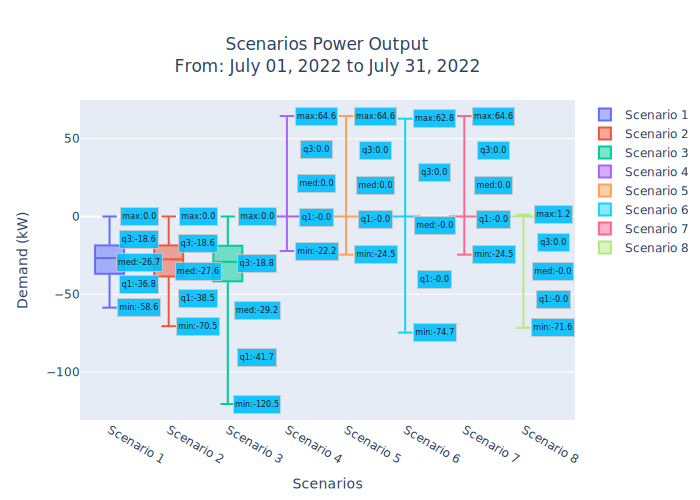
\includegraphics[width=0.7\linewidth]{Fig/Option_3/4_Scn_Output_Run_3_Jul_01_2022_to_Jul_31_2022}
				\caption{\footnotesize  Power Measured from the Meter for the Month of July}
				\label{fig:4scnoutputrun2jul012022tojul312022}
			\end{figure}
		\end{frame}
		
		\begin{frame}
			\frametitle{Results}
			\begin{figure}
				\centering
				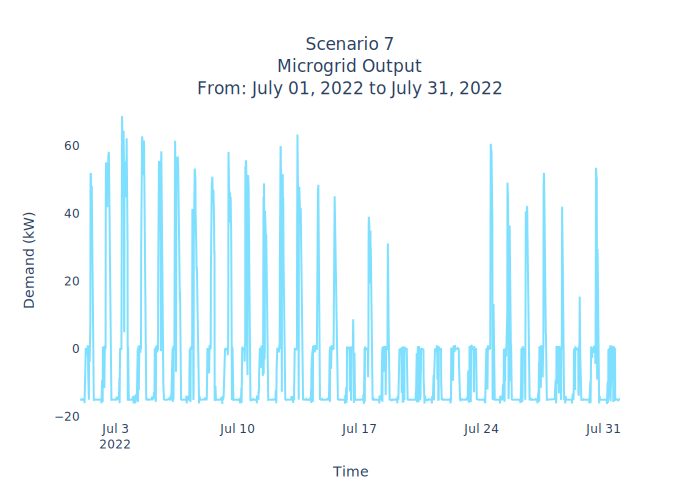
\includegraphics[width=0.7\linewidth]{Fig/Option_3/4_Scenario_7_Run_3_Mg_Output_Jul_01_2022_to_Jul_31_2022.pdf}
				\caption{\footnotesize Peak Shaving Failure after Battery Depletion (Level 2 Charging, 500 kWh BESS)}
				\label{fig:scenario3peakshaving}
			\end{figure}
		\end{frame}
		
		\begin{frame}
			\frametitle{Results}
			\begin{figure}
				\centering
				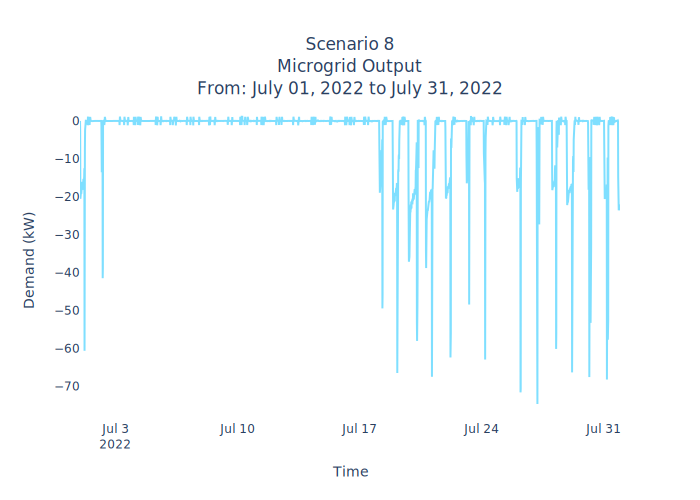
\includegraphics[width=0.7\linewidth]{Fig/Option_3/4_Scenario_8_Run_3_Mg_Output_Jul_01_2022_to_Jul_31_2022.pdf}
				\caption{\footnotesize Peak Shaving Failure after Battery Depletion (Level 2 and Level 3 Charging, 500 kWh BESS)}
				\label{fig:scenario4peakshaving}
			\end{figure}
		\end{frame}
		
		\begin{frame}
			\frametitle{Results}
			\begin{table}
				\caption{Microgrid Utility Prices and CO\textsubscript{2} Emissions Output under Different Pricing Scenarios and Pricing Structures}
				\centering
				\large
				\begin{tabular}{rrrrr}
\toprule
 Scenario &  Demand Charges (\$) &  Energy Charges (\$) &  Total Cost (\$) &  Emissions \\
\midrule
        1 &                6616 &               22736 &           29352 &         34 \\
        2 &                8196 &               24607 &           32803 &         37 \\
        3 &                3887 &                1556 &            5443 &          5 \\
        4 &               11744 &                5841 &           17585 &         23 \\
        5 &                5133 &                3256 &            8389 &          7 \\
        6 &               11329 &                8091 &           19420 &         14 \\
        7 &                5022 &                3396 &            8418 &          7 \\
        8 &               11400 &                8075 &           19475 &         14 \\
\bottomrule
\end{tabular}

				\label{tab:emissions}
			\end{table}
		\end{frame}
		
		\begin{frame}
			\frametitle{Results}
			\begin{figure}
				\centering
				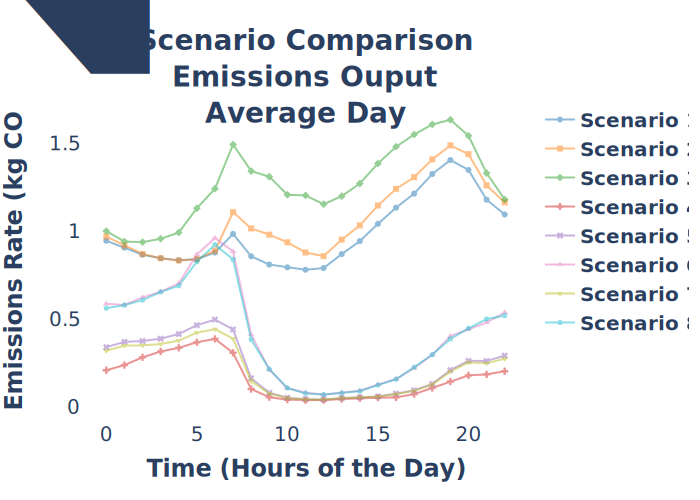
\includegraphics[width=0.7\linewidth]{Fig/Option_3/emissions_scenario_comparison_run_3_large_font.pdf}
				\caption{Microgrid CO\textsubscript{2} Emissions Outputs Averages During Times of Day: Adding a microgrid significantly reduces CO\textsubscript{2} Emissions compared to the non-microgrid scenarios of 1, 2, and 3.}
				\label{fig:emissions_output}
			\end{figure}
		\end{frame}
\section{Conclusions and Future Work}		
	\Large
	\begin{frame}[allowframebreaks]
		\frametitle{Conclusions and Future Work}
		\begin{itemize} \large
			\item \textbf{Transportation Microgrids Benefits:}
			\begin{itemize} \large
				\item Reduced Electricity Costs:
				\begin{itemize} \large
					\item Load-Following Algorithm: \$23,000 - \$24,000 annual savings
					\item Cost of Demand Saved: Follows total cost trend (around \$3,000)
					\item Cost of Energy Saved: Follows total cost trend (around \$21,000)
				\end{itemize}
				\item Reduced CO\textsubscript{2} Emissions: 
				\begin{itemize} \large
					\item Load-Following Algorithm: 67\% - 85\% reduction (30 tons CO\textsubscript{2}/year)
				\end{itemize}
			\end{itemize}
			\item \textbf{Key Considerations for Optimization:}
			\begin{itemize} \large
				\item Balance Clean Energy Sources (Solar/Wind) with Load:
				\begin{itemize} \large
					\item Level 2 chargers: manageable for office buildings
					\item Level 3 fast chargers: require additional clean energy sources
				\end{itemize} \large
				\item Net Energy Metering Policy:
				\begin{itemize} \large
					\item  Incentivizes  low CO\textsubscript{2} load-following operation of a microgrid instead of peak-shaving
				\end{itemize}
				\item Battery Capacity (BESS):
				\begin{itemize} \large
					\item Increased capacity for extreme solar outages is expensive with diminishing returns on CO\textsubscript{2}/cost savings
					\item Requires additional solar power for full battery charge during daylight
				\end{itemize}
			\end{itemize}
			\framebreak
			\item \textbf{Effective Microgrid Planning:}
			\begin{itemize} \large
				\item Requires all three aspects:
				\begin{itemize} \large
					\item Clean Energy Generation
					\item Energy Storage
					\item Load Management
				\end{itemize}
			\end{itemize}
		\item \textbf{Future Work}
			\begin{itemize} \large
				\item Explore advanced control strategies for optimizing electric costs and CO\textsubscript{2} emissions in transportation-microgrid.
				\item Assess effects of new net energy metering policy in California on BESS system value.
				\item Analyze impact of different time-of-use (TOU) rates in California on electric costs and CO\textsubscript{2} emissions.
				\item Investigate methods to maximize clean energy utilization and minimize grid power during high CO\textsubscript{2} times.
			\end{itemize}
		\end{itemize}
	\end{frame}
		
%		\begin{frame}
%			\frametitle{Conclusions and Future Work}
%			\begin{itemize}
%				\item Transportation-microgrids mitigate electrical costs and emissions associated with EV charging infrastructure
%				\item Load-following transportation-microgrids yield annual savings of \$23,000 to \$24,000, despite additional EV charger demand
%				\item Similar savings observed with varying demand and a sufficiently large Battery Energy Storage System (BESS)
%				\item Cost of demand and energy saved align with total cost trends (\$3,000 and \$21,000 respectively)
%				\item Load-following microgrids reduce CO\textsubscript{2} emissions by 67\% to 85\% (approximately 30 tons of CO\textsubscript{2})
%				\item Additional clean energy sources should be added to a microgrid when EV chargers are added, especially with Level 3 fast chargers
%				\item New net energy metering policies enhance economic viability of low CO\textsubscript{2} emission load-following algorithms
%				\item Increasing battery capacity does not guarantee improved performance, requires additional solar power for CO\textsubscript{2} reduction
%				\item Sensible microgrid planning necessitates clean energy generation, energy storage, and load management
%				\item Careful consideration of battery and generation capacity, along with electricity pricing structures, is crucial for optimization
%			\end{itemize}
%		\end{frame}
	
	\begin{frame}
		\frametitle{\null}
		\centering
		\Huge
		Questions?
	\end{frame}
	
	\begin{frame}
		\frametitle{\null}
		\centering
		\Huge
		Thank You
	\end{frame}
	
	\begin{frame}[allowframebreaks]
		\frametitle{References}
		\nocite{*}
		\bibliographystyle{IEEEtran}
		\bibliography{cite}
	\end{frame}
\end{document}
